\section{Materials and Methods}
    
\subsection{Description of the Dataset}

We used publicly available EEG recordings of \numSubjects~participants (\numFemaleSubjects~female; \numRightHandedSubjects~right-handed; mean age = \meanAge~years, SD = \sdAge~years) from a study that investigated the effects of mindfulness-based training on performance in a motor imagery BCI task \citep{Stieger2021_dataset}. Participants first completed a baseline BCI training session and then were randomly assigned to an 8-week mindfulness intervention (n = \numMBSRSubjects; \numFemaleMBSRSubjects~female; \numRightHandedMBSRSubjects~right-handed; mean age = \meanAgeMBSR, SD = \sdAgeMBSR) and a wait-list control condition of the same length (n = \numControlSubjects; \numFemaleControlSubjects~female; \numRightHandedControlSubjects~right-handed; mean age = \meanAgeControl, SD = \sdAgeControl). After eight weeks, participants returned to the lab for \numFollowUpSessionsMin-\numFollowUpSessionsMax~more sessions of BCI training (Fig. \ref{fig:dataset_overview}A). All experiments were approved by the institutional review boards of the University of Minnesota and Carnegie Mellon University. Informed consent was obtained from all participants.

\subsection{Experimental Procedure}

During each BCI session, participants performed imaginary movements (opening and closing) of their hands to control a cursor, which was displayed on the screen in front of them in the BCI2000 system \citep{BCI2000_Schalk2004}. Each session included three tasks: (1) horizontal cursor control task (via imaginary movements of the left or right hand), (2) vertical cursor control task (down: voluntary rest, up: imaginary movement of both hands), (3) 2D control task (the targets were reachable through one of the previous strategies, but the cursor moved in both directions). Each task included 150 trials, and the number of trials was balanced across classes for both 1D and 2D control tasks. In the current study, we only analyzed the data from the first (horizontal cursor control) task.

\medskip

The structure of all trials is shown in Fig. \ref{fig:dataset_overview}B. First, participants saw a blank screen during the inter-trial interval of 2 s. Then, a bar appeared on one of the sides of the screen, indicating the target action to execute. After 2 seconds of target presentation, a cursor (circle) appeared in the middle of the screen, and its position was calculated based on the EEG data acquired in real time. Trials ended either when the cursor reached any side of the screen (not necessarily the target one) or after the timeout when 6 seconds passed without any target being reached.

\medskip

Feedback was presented with a cursor, whose position was updated in real time based on the EEG power in the mu (\muLow-\muHigh~Hz) frequency range. Power was calculated based on an autoregressive model of order 16 fitted to the most recent 160 ms of the EEG data after applying small Laplacian transform to channels C3 and C4 (using the closest neighboring channels FC3, CP3, C1, C5 and FC4, CP4, C2, C6, respectively). The horizontal position of the cursor was determined by the lateralization of mu power (C4 -- C3), while the vertical position reflected the total mu power (C4 + C3). Feedback values were re-calculated every 40 ms and normalized by subtracting the mean and dividing over the standard deviation. The mean and the standard deviation were constantly updated based on the last 30 seconds of data. More details about the experimental procedure can be found in \citep{Stieger2021_dataset}.

\begin{figure}[htbp]
    \centering
    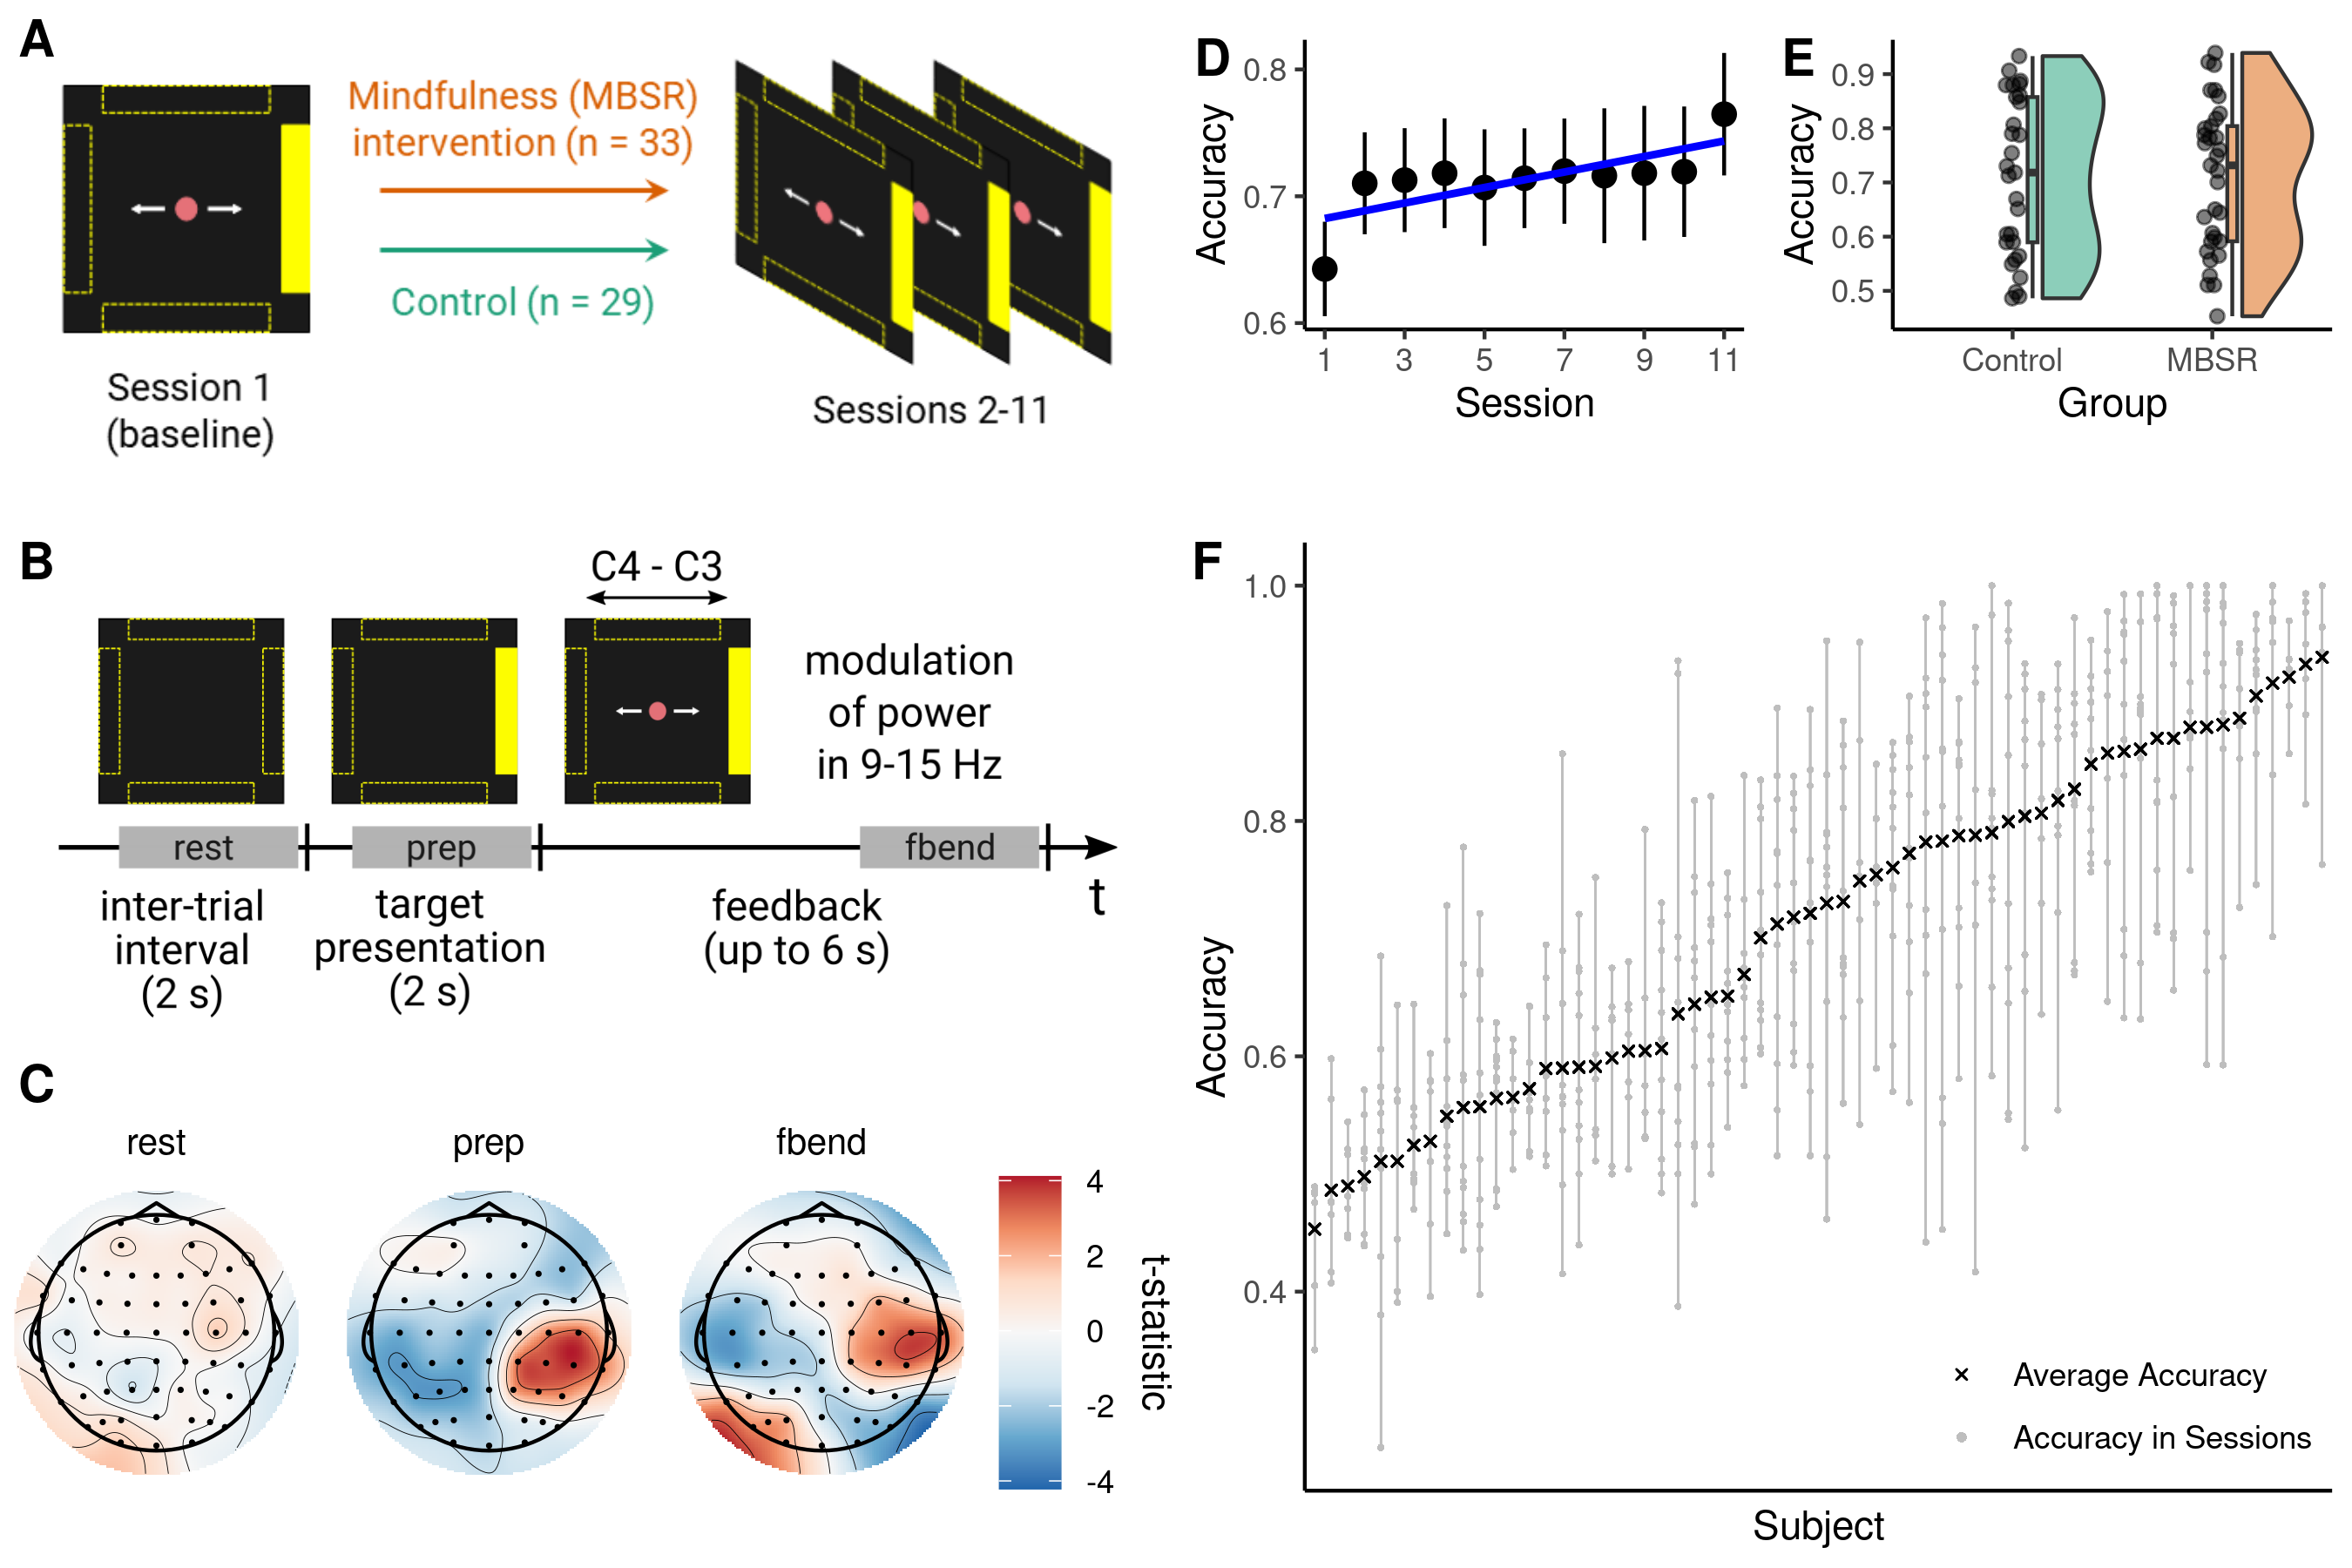
\includegraphics[width=\textwidth]{fig1-dataset-overview.png}
    \caption{Overview of the publicly available dataset from \citep{Stieger2021_dataset}: structure of the BCI training and performance of the participants. (A) Participants were assigned to MBSR (mindfulness-based stress reduction) and control groups and completed up to 11 sessions of cursor control training. (B) Trial structure of the horizontal cursor control task with time windows of interest highlighted. Participants performed imaginary movements of their left and right hands to control a cursor, whose position was calculated based on the values of mu power at Laplace-transformed channels C3 and C4 in real time. (C) Channel-wise t-statistic of difference in mu power between trials that involved imaginary movements of the right and left hand. While no difference in mu power was observed during the resting-state period, effects emerged over sensorimotor areas during target presentation, accompanied by effects over visual areas due to the movement of the cursor during the feedback period. (D) Dynamics of group-average performance reflect improvement over the course of the training. Error bars reflect the standard error of the mean. (E) No difference in average performance in the horizontal cursor control task was observed between groups. (F) High variability of performance in the individual sessions was observed and accounted for in the analyses. Subjects are ordered according to their average accuracy. Vertical bars depict subject-specific ranges of accuracy.}
    \label{fig:dataset_overview}
\end{figure}

\subsection{EEG Acquisition}

EEG was acquired using SynAmps RT amplifiers and Neuroscan acquisition software (Compumedics Neuroscan, VA). Data were recorded with a sampling frequency of 1 kHz and band-pass filtered between 0.1 and 200 Hz with an additional notch filter at 60 Hz. EEG data were acquired from \numChannelsOrig~channels with the following locations according to the 10-5 system: \channelsOrig. AFz was used as the ground electrode, while the reference electrode was located between Cz and CPz.

\subsection{Preprocessing}

EEG preprocessing and analyses were performed in MATLAB R2022b (The MathWorks; RRID: SCR\_001622) using custom scripts employing functions from EEGLAB 2021.0 (\cite{EEGLAB_Delorme2004}; RRID: SCR\_007292), BBCI \citep{Blankertz2016}, Brainstorm (\cite{Brainstorm_Tadel2011}; RRID: SCR\_001761), MVGC (\cite{MVGC_Barnett2014}; RRID: SCR\_015755) and METH (Guido Nolte; RRID: SCR\_016104) toolboxes. For source space visualizations, we utilized functions from \citep{HaufeEwald2019}.

\medskip

First, trials were concatenated to restore continuous segments of data accounting for breaks during the recording. Then, EEG time series were downsampled to \downsampleFreq~Hz, and channels CB1 and CB2 were removed as they are not part of the 10-10 system. A semi-automatic identification of bad trials, channels, and components was applied as follows. Trials and channels were rejected if the z-score of power within 1-45 Hz was higher than three in at least 5\% of trials for a certain channel or in at least 5\% of channels for a certain trial. This procedure was performed recursively until nothing could be rejected. Additionally, we used the clean\_rawdata EEGLAB plugin to reject channels if one of the following conditions was met: (1) the variance of the channel data was near zero for at least five seconds, (2) the ratio of the power of the line noise and power of the signal below 50 Hz exceeded 4, or (3) the correlation of the channel data with an interpolated estimate based on the data from neighboring channels was less than 0.8. After the removal of bad trials and channels, EEG data were re-referenced to the common average reference and filtered with a forward-backward second-order high-pass Butterworth filter with a cutoff frequency of 1 Hz. Then, we applied independent component analysis (ICA) based on the FastICA approach \citep{FastICA_Hyvaerinen1999} and used ICLabel \citep{ICLabel_PionTonachini2019} for distinguishing ICA components of different types: brain, muscle, eye, heart, line noise, and channel noise. Based on the output of ICLabel, components that explained 95\% of the variance in the data were rejected if their probability of originating from the brain was less than 20\%, and other components were rejected only if their probability of belonging to one of the non-brain classes was at least 80\%.

\medskip

Results of the automatic preprocessing were verified through visual inspection of power spectra in sensor space as well as topographic maps and power spectra of kept and rejected ICA components. Overall, \numSessionsExcluded~sessions were excluded from analysis due to poor data quality. Then, we removed previously identified bad trials, channels, and ICA components from the raw EEG data that were not high-pass filtered. The removed channels were interpolated, and EEG time series were downsampled to \downsampleFreq~Hz. DC offset was removed by subtracting the mean of the signal within continuous data segments. The resulting data were used for the analyses described below.

\subsection{Overview of the Analyses}

In this section, we provide a brief overview of the performed analyses. The detailed description of the processing steps is presented in the subsequent sections.

\medskip

In the current study, we only analyzed the data from the first (horizontal cursor control) task, which was based on the imaginary movements of the left or right hand. Additionally, we combined the data from both participant groups since a previous analysis of the same dataset has shown that the mindfulness intervention did not affect the performance in the horizontal cursor control task \citep{Stieger2020_analysis}.

\medskip

We estimated the values of SNR of the mu rhythm (in sensor and source space) and phase synchronization between sensorimotor areas (source space only) in order to investigate their relationship with BCI performance and changes over time. For both of the analyses, we focused on the same [0.49, 1.99] s window of the inter-trial interval (labeled as rest in Fig. \ref{fig:dataset_overview}B). During this interval, participants did not perform any task similar to a typical resting-state recording. Previous studies often used resting-state data to predict BCI performance in subsequent training sessions. Additionally, we investigated differences in mu power during the [0.49, 1.99] s window of the target presentation interval as well as the [-1.51, -0.01] s window relative to the end of the feedback interval (Fig. \ref{fig:dataset_overview}C). The performance in the BCI task (later referred to as accuracy) was assessed with the percentage of correct trials among those that did not end due to timeout. Trials were considered correct if the cursor reached the target side of the screen.

\medskip

In the sensor space analysis, we applied the small Laplacian transform by subtracting the mean of the neighboring channels (FC3, C5, C1, CP3 or FC4, C6, C2, CP4) from data at channels C3 and C4. The same transform was used during the experiment for calculating the feedback values in real time. Then, we estimated the SNR of the mu rhythm (\muLow-\muHigh~Hz) and correlated it with the BCI performance similar to \citep{Blankertz2010}. Additionally, we examined longitudinal changes in SNR across sessions to find out whether the BCI training affected the SNR of the mu rhythm.

\medskip

In the source space analysis, we estimated the SNR of the mu rhythm and phase synchronization between the sensorimotor regions of interest (ROIs) to obtain higher spatial specificity. The time courses of activity in each ROI were computed through inverse modeling and subsequent aggregation of reconstructed time series of source dipoles within the ROI. Various methods for inverse modeling and extraction of ROI time series are used in the literature with few guidelines for preferring one over the other. Therefore, we combined several widely used data-driven and data-independent approaches in a multiverse analysis \citep{Steegen2016} to investigate the robustness of SNR and PS values as well as related statistical effects (e.g., on BCI performance) to the selection of the pipeline (Fig. \ref{fig:pipeline_overview}A).

\subsection{Forward Model}

We used the ``New York Head'' forward model \citep{Huang2016NYHead}, which was derived using the finite element method based on the ICBM152 anatomical template \citep{Fonov2009, Fonov2011}. The model contains several lead field matrices calculated for different numbers and orientations of the source dipoles (later referred to as sources). We used the lead field matrix for \numVoxels~sources with fixed orientations perpendicular to the cortical surface. Since channels PO5 and PO6 were not included in the precomputed lead field, we excluded them before source space analysis. The common average reference transform was applied to the lead field matrix to match the preprocessing of the EEG data.

\subsection{Inverse Modeling}

We used two inverse solutions with different underlying assumptions: eLORETA \citep{eLORETA_PascualMarqui2007} and linearly constrained minimal variance (LCMV) beamformer \citep{LCMV_VanVeen1997}. For both approaches, we used the implementation from the METH toolbox (Guido Nolte; RRID: SCR\_016104) with minor modifications from \citep{HaufeEwald2019}. The regularization parameter was set to \inverseRegFactor~and the identity matrix was used as the noise covariance matrix. 

\medskip

eLORETA is a data-independent approach that belongs to the family of weighted minimum norm inverse solutions and provides zero source localization error \citep{PascualMarqui2011}. In the described setting, this approach is also data-independent. In contrast, LCMV is a data-driven method and is fit to the covariance matrix of the data. We averaged covariance matrices for both imaginary movements and calculated a separate LCMV beamformer for each subject and session.

\subsection{Extraction of ROI Time Series}

After the inverse modeling, one obtains a reconstructed time series of activity for each source. Taking into account the spatial resolution of EEG, it is reasonable to reduce the dimensionality of the source space. The common approach is to aggregate time courses of activity of sources within each ROI into a single or several time series. Yet, multiple aggregation methods exist in the literature, and there is no consensus in the community on the most appropriate method. In particular, previous studies have used averaging \citep{Babiloni2005}, averaging with sign flip (AVG-F; \cite{Lai2018}), singular value decomposition (SVD; \cite{Rubega2019}), etc. In the current analysis, we considered AVG-F and SVD to compare data-independent and data-driven approaches.

\medskip

For both approaches, the time series of activity for all sources within the ROI are concatenated to form a matrix. By fitting SVD, one decomposes the multivariate time series of activity into components sorted by the explained variance of the reconstructed source data. Then, a few first components are selected to represent the activity of the whole ROI. We considered either only the first (1SVD) or the first three components (3SVD) as, e.g., in \citep{Rubega2019, Pellegrini2023} or \citep{Vidaurre2020, Pellegrini2023}, respectively. 

\medskip

Alternatively, AVG-F assigns equal weights to all sources within the ROI, and a sign flip is applied to some sources to prevent the cancellation of the activity of dipoles with opposite orientations. To determine the sources that should be flipped, SVD is applied to the leadfield of sources within the ROI to find the dominant orientation of source dipoles. If the angle between the orientation of the dipole and the dominant orientation is larger than 90 degrees, the time series corresponding to this dipole is flipped (that is, multiplied by a negative one). We used the implementation of sign flip from Brainstorm \citep{Brainstorm_Tadel2011}. Fig. \ref{fig:pipeline_overview}C shows 1SVD and AVG-F weights for all sources within the sensorimotor ROIs based on the data of an exemplary subject.

\subsection{Anatomical and Task-Based Definitions of ROIs}

All the analyses in the source space were performed for four sensorimotor ROIs --- pre- and postcentral gyri of both hemispheres --- either according to their definitions in the Harvard-Oxford atlas \citep{Frazier2005HOA, Desikan2006HOA, Makris2006HOA, Goldstein2007HOA, Jenkinson2012FSL} or reduced to a group of task-relevant sources (Fig. \ref{fig:pipeline_overview}B). To select a subset of sources that contribute the most to the observed task-related changes in the brain activity, we applied a mask in source space derived from the common spatial pattern (CSP) transformation \citep{Koles1990, Ramoser2000}. CSP was applied to the sensor space data filtered in the \muLow-\muHigh~Hz range for extracting spatial filters that explain the most difference in EEG power between the two imaginary movements. For this purpose, we used the EEG data during the [0.49, 1.99] s window of the target presentation interval (labeled as prep in Fig. \ref{fig:dataset_overview}B). Covariance matrices of the signal were calculated for each subject, session, and imaginary movement separately. Then, for each subject and session, covariance matrices corresponding to different imaginary movements were normalized to make the trace of their average equal to one. The normalization allowed us to exclude the difference in signal power between subjects and sessions while preserving the within-session difference in power between channels and imaginary movements. Normalized covariance matrices were averaged over all subjects and sessions and then used to obtain one set of CSP filters and patterns for all participants. CSP patterns were then source reconstructed with eLORETA. A threshold based on \cspSourceThreshold th percentile of activity strength was applied to select the most responsive sources, which formed the resulting source mask. The mask was applied to the anatomical definitions of sensorimotor ROIs to obtain a task-based reduced representation.

\subsection{Filtering}

Due to the 1/f shape of the M/EEG power spectra, lower frequencies ($<$ 7 Hz) might have higher power and overshadow mu oscillations in covariance calculations. By filtering the data in a narrow frequency band, one makes sure that data-dependent methods (LCMV, SVD) are not affected by frequencies outside of the target band. At the same time, data-independent methods (eLORETA, AVG-F) are not affected by filtering.

\medskip

To investigate how filtering in a narrow frequency band affects data-dependent methods for inverse modeling and extraction of ROI time series, we considered two cases: broadband with no filtering (BB) or band-pass filtering in the \muLow-\muHigh~Hz band (NB). A forward-backward fourth-order Butterworth filter was applied before restricting the data to the time windows of interest and applying the inverse modeling. Since the recording contained breaks, \mirrorSeconds~seconds of data in the beginning and the end were mirrored to minimize filtering-related artifacts at the edges of continuous data segments. Separate LCMV beamformers and sets of SVD weights were calculated for broadband and narrowband data.

\subsection{SNR}

SNR was estimated as the ratio of the total power and the power of the aperiodic component of the signal in the \muLow-\muHigh~Hz frequency range as follows:

\begin{equation}
    \text{SNR [dB]} = 10 \cdot \log_{10} \frac{P_{total}}{P_{aperiodic}}
\end{equation}

The aperiodic component of the signal was estimated using FOOOF (Fig. \ref{fig:pipeline_overview}D; \cite{FOOOF_Donoghue2020}) with the following set of parameters: \fooofFitRangeLow-\fooofFitRangeHigh~Hz fit range, \fooofPeakWidthMin-\fooofPeakWidthMax~Hz as limits of peak width, and \fooofNumPeaksMax~as the maximal number of peaks. Since it is not possible to fit an aperiodic component for the data that was already band-pass filtered in a narrow frequency range, values of SNR for pipelines that involved filtering were copied from the corresponding broadband pipeline, which had all the other steps unchanged. Values of SNR were estimated in the same manner for the sensor space data after the Laplacian transform and in the source space, later referred to as Laplace SNR and ROI SNR, respectively.

\subsection{Phase Synchronization}

To estimate phase synchronization between time series of activity in ROIs, we employed three measures: imaginary part of coherency (ImCoh; \cite{Nolte2004}), lagged coherence (LagCoh; \cite{PascualMarqui2011}), and coherence (the absolute value of coherency). ImCoh and LagCoh are insensitive to all zero-lag interactions, including the spurious ones caused by the volume conduction. However, it may be hard to interpret correlations between performance and phase synchronization as measured by ImCoh and LagCoh. Both measures depend on the strength and the phase lag of the interaction between neuronal populations. If ImCoh or LagCoh is correlated with performance, it is not entirely clear whether the strength or the phase lag of interaction drives the correlation. At the same time, coherence is supposed to solely reflect the strength of an interaction, but is prone to the effects of volume conduction and might be spurious. To combine interpretability and robustness to spurious zero-lag interactions, we have considered all of these PS measures and looked at whether the observed effects are consistent between them.

\medskip

We computed the phase synchronization via the Fourier transform for broadband pipelines using the Hamming window and \fftSegLength~s segments from different trials (frequency resolution = \fftFreqRes~Hz) and averaged the absolute values of PS measures across frequencies of interest (\muLow-\muHigh~Hz). If the data were filtered in the \muLow-\muHigh~Hz range, we calculated the phase synchronization via the analytic signal obtained using the Hilbert transform. These approaches were shown to have a negligible difference within the frequency band of interest for Gaussian distributed data \citep{Nolte2020}. In the case of several SVD components per ROI, PS values were first computed for each pair of the SVD components, then the absolute values of PS were averaged. Furthermore, absolute PS values were averaged over within-hemisphere and across-hemisphere edges as shown in Fig. \ref{fig:pipeline_overview}E, which resulted in two values (i.e., within and across-hemisphere connectivity) per session for each subject similar to \citep{Vidaurre2020}.

\medskip

Since changes in SNR of oscillations in the frequency band of interest lead to spurious changes in PS due to either more or less accurate phase estimation \citep{MuthukumaraswamySingh2011}, we applied a correction for SNR in the statistical analyses.

\subsection{Multiverse Analysis}

Overall, in the current multiverse analysis, we considered \numPipelines~pipelines based on all possible combinations of methods for the aforementioned processing steps (Fig. \ref{fig:pipeline_overview}A). By selecting these pipelines, we aimed to assess the effects of data-independent (eLORETA, AVG-F, BB, anatomical ROIs) and task- or subject-dependent (LCMV, SVD, NB, task-based ROIs) methods on the estimated values of SNR and connectivity, their relationship with BCI performance, and changes over time. For each pipeline, we estimated the values of SNR as well as within- and across-hemisphere PS. Then, we tested their relationship with performance and changes over time, as described below.

\begin{figure}[htbp]
    \centering
    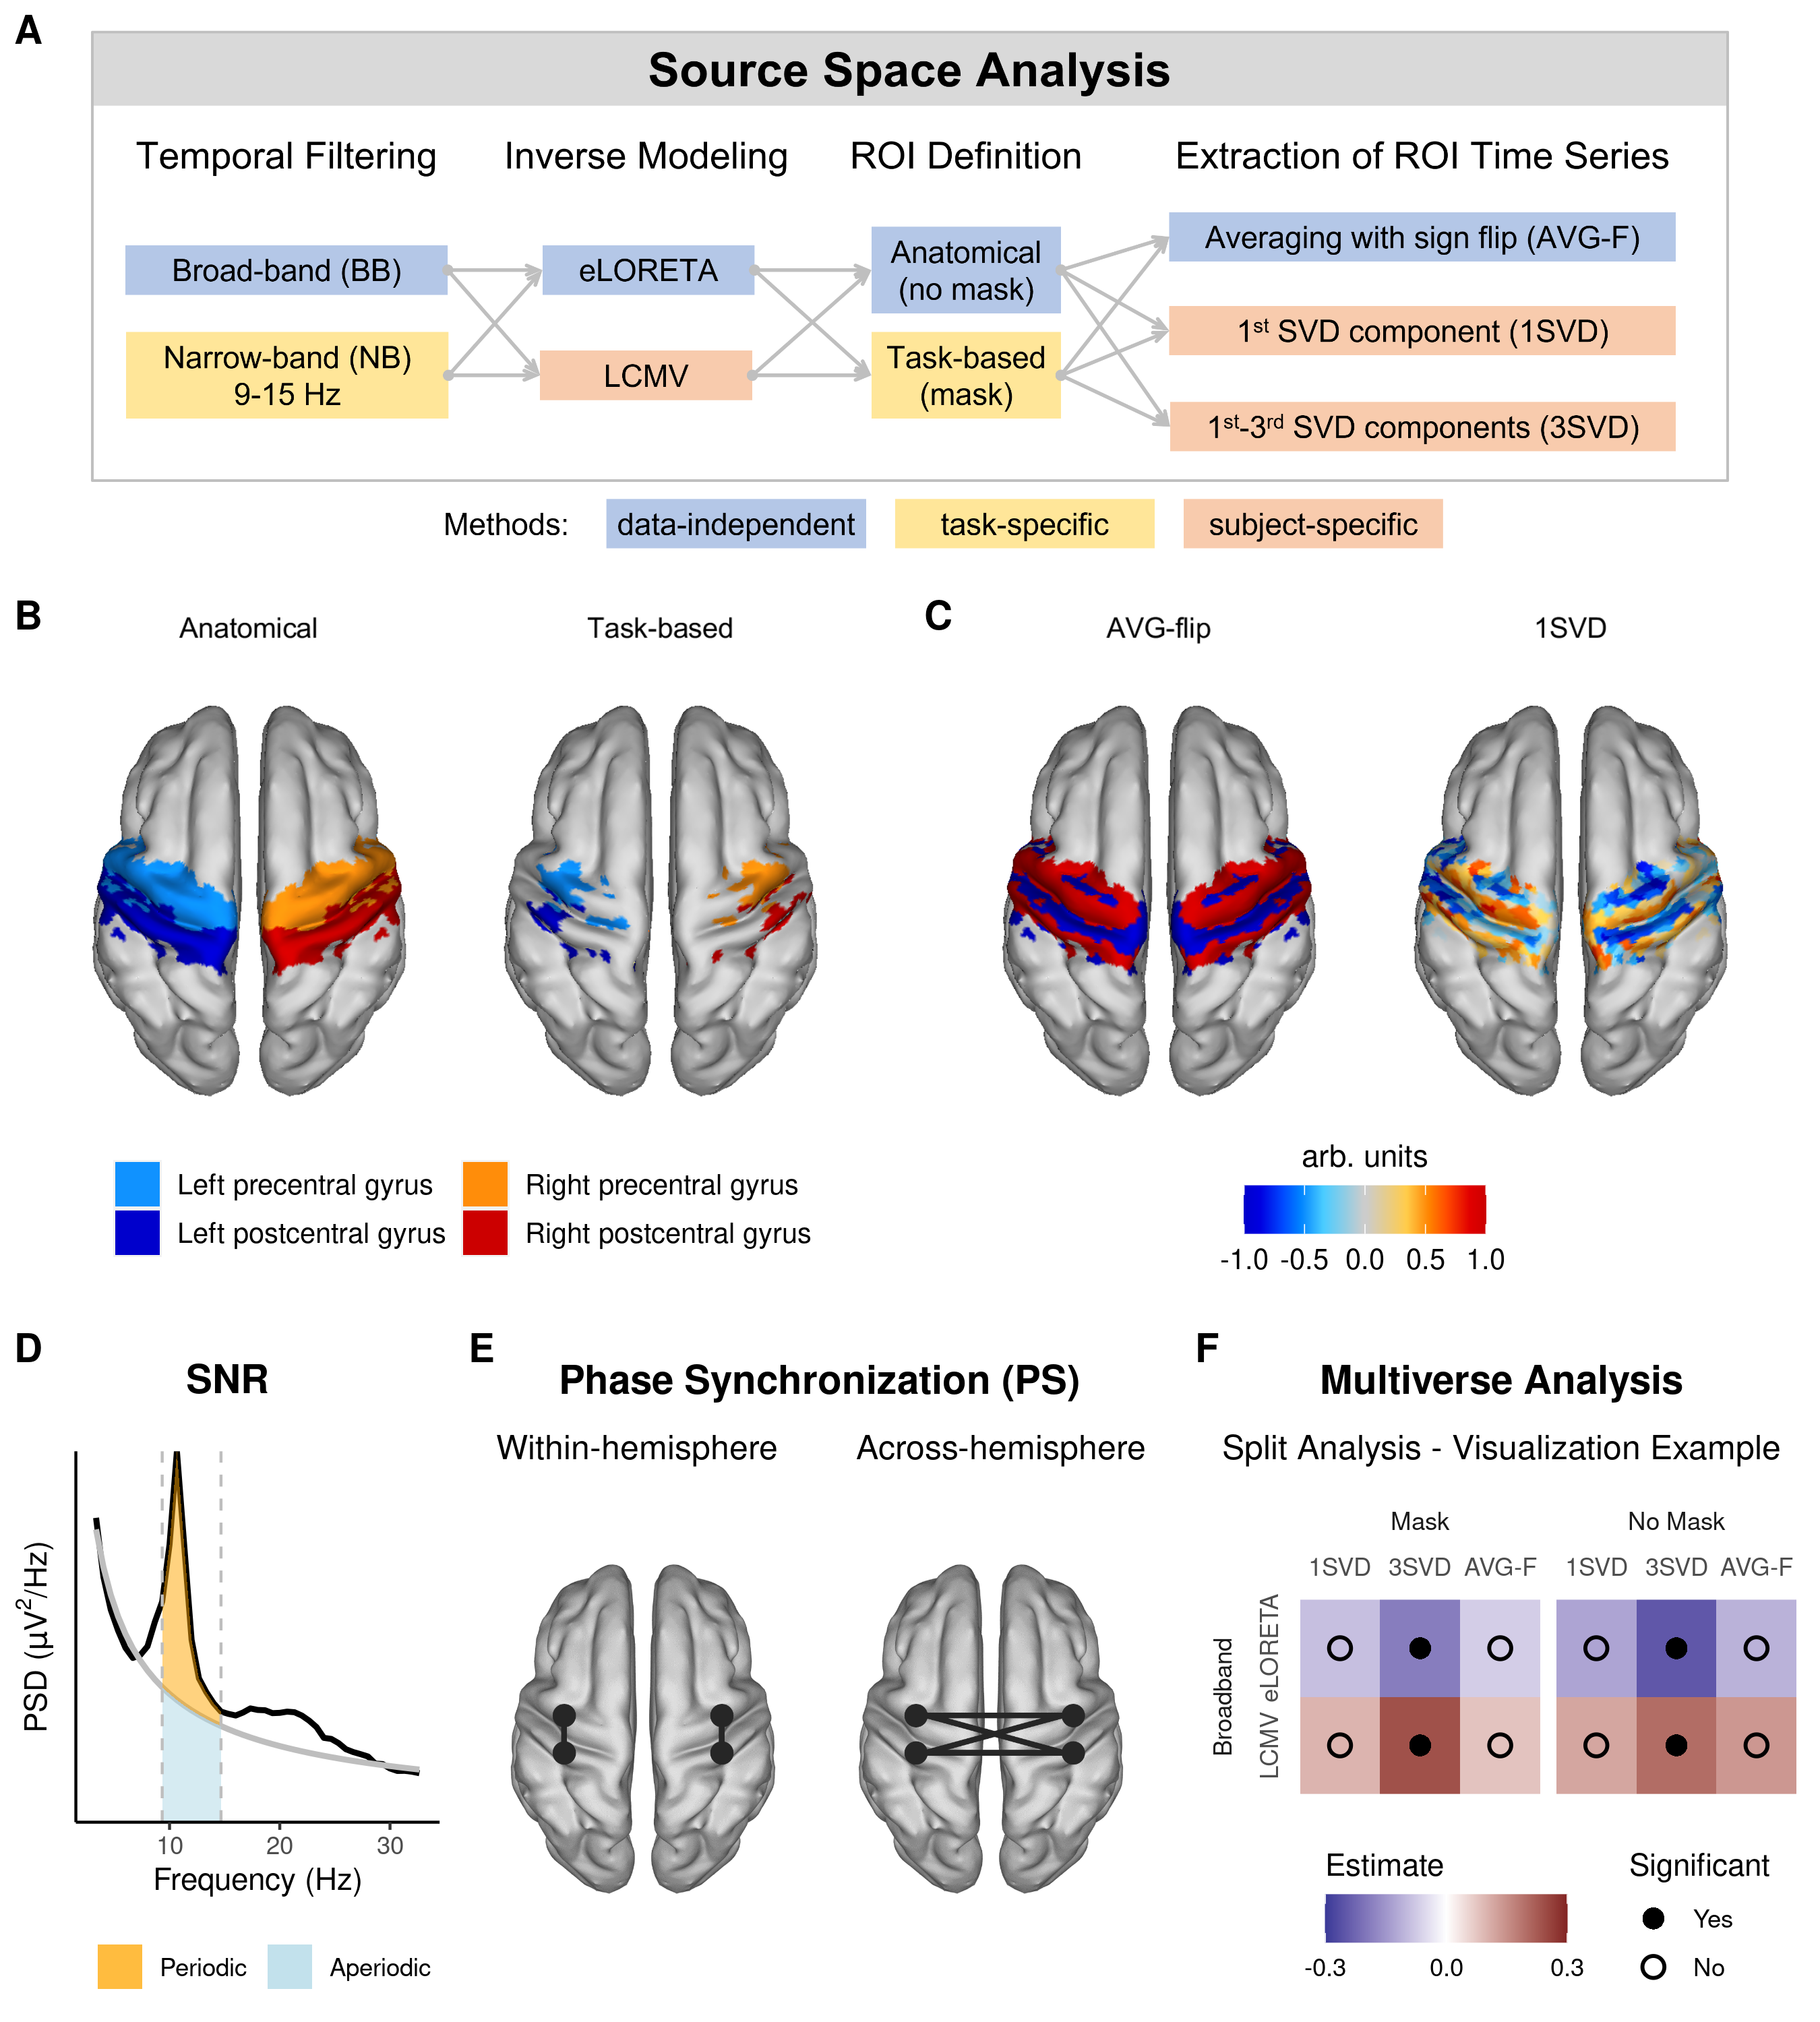
\includegraphics[width=\textwidth]{fig2-pipeline-overview.png}
    \caption{Overview of the multiverse analysis of SNR and phase synchronization in the source space. (A) \numPipelines~combinations of the data-independent and task- or subject-specific methods were used in the current analysis. (B) Anatomical (No Mask) and task-based (Mask, derived using CSP) definitions of sensorimotor ROIs. (C) AVG-F and 1SVD weights for all sources within sensorimotor ROIs for an exemplary subject. (D) SNR was estimated as the ratio of the total (periodic + aperiodic) power and the power of the aperiodic component in the \muLow-\muHigh~Hz frequency range. The gray line depicts the 1/f fit obtained with FOOOF. (E) Phase synchronization values were averaged over the within-hemisphere and across-hemisphere interactions between sensorimotor ROIs. (F) Statistical results were aggregated in a table to assess the robustness of effects to the selection of the pipeline. Estimated correlations (between-subject effect) or beta weights (within-subject effect) were coded with color, and the significance of the effects was indicated by filled black dots.}
    \label{fig:pipeline_overview}
\end{figure}

\subsection{Statistical Analysis}

Statistical analysis was performed in R 4.2.2 \citep{R_Core}. We used one-sample t-tests to analyze differences in mu power between trials corresponding to the imaginary movements. Also, we used Welch's two-sample t-test to check for group differences in performance and SNR. To assess the between-subject effects of SNR or phase synchronization on BCI performance, we correlated accuracy and a predictor variable (SNR or PS) after averaging them over all sessions for each subject. Within-subject effects of SNR and PS on accuracy as well as changes in SNR and PS over time were assessed with linear mixed-effect (LME) models using lme4 \citep{R_lme4} and lmerTest \citep{R_lmerTest} packages. The values of continuous variables were normalized before fitting the LMEs by subtracting the mean and dividing over the standard deviation. The denominator degrees of freedom in the LMEs were adjusted according to Satterthwaite's method \citep{Satterthwaite1946}. P-values less than \pSignificant~were considered significant. The LME models that correspond to the research questions (relationship between SNR or PS and BCI performance, changes in SNR and PS over time, and effects of different processing methods on SNR and PS) are presented in Table \ref{tab:stat_formula}. Additionally, we used linear mixed models to investigate the relationship between SNR and PS values.

\begin{table}[htbp]
    \small
    \centering
    \resizebox{\linewidth}{!}{\begin{tabular}{llc}
        \toprule
        \textbf{Effect} & \textbf{Model} \\
        \midrule
        \multicolumn{3}{l}{\textit{Relationship between SNR and Phase Synchronization (PS) Values}} \\
        SNR $\rightarrow$ PS & \formulaSNRConnectivity & ($\ast$) \\
        \midrule
        \multicolumn{3}{l}{\textit{Relationship between SNR or PS and BCI Performance (Accuracy)}} \\
        SNR $\rightarrow$ Acc. & \formulaAccuracySNR & ($\ast$) \\
        PS $\rightarrow$ Acc. & \formulaAccuracyConnectivity & ($\ast$) \\ 
        PS $\rightarrow$ Acc. $|$ SNR & \formulaAccuracyConnectivitySNR & ($\ast$) \\
        \midrule
        \multicolumn{3}{l}{\textit{Longitudinal Changes in Accuracy, SNR, and Phase Synchronization}} \\
        Session $\rightarrow$ Acc. & \formulaAccuracySession & \\
        Session $\rightarrow$ SNR & \formulaSNRSession & ($\ast$) \\ 
        Session $\rightarrow$ PS & \formulaConnectivitySession & ($\ast$) \\ 
        Session $\rightarrow$ PS $|$ SNR & \formulaConnectivitySessionSNR & ($\ast$) \\
        \midrule
        \multicolumn{3}{l}{\textit{Effects of the Processing Methods on the Estimated SNR and Phase Synchronization}} \\
        Methods $\rightarrow$ SNR & \formulaSNRProcessing & \\
        Methods $\rightarrow$ PS & \formulaConnectivityProcessing & \\
        Methods $\rightarrow$ PS $|$ SNR & \formulaConnectivityProcessingSNR & \\
        \bottomrule
        \multicolumn{3}{l}{($\ast$) random effect of the processing pipeline (1 $|$ Pipeline) was added in the joint multiverse analysis.}
    \end{tabular}}
    \caption{Linear mixed-effects models that were used for the assessment of the effects of interest. Notation $\text{X} \rightarrow \text{Y} ~|~ \text{Z}$ corresponds to the effects of $\text{X}$ on $\text{Y}$, controlled for $\text{Z}$. Acc., ROI, and Inv. stand for Accuracy, Extraction of ROI Time Series and Inverse Modeling, respectively. Random slopes were added to the models as long as they converged for all of the considered pipelines.}
    \label{tab:stat_formula}
\end{table}

\medskip

For the multiverse analysis, we have considered two approaches: split and joint analysis. In the split analysis, we fitted a separate mixed model for each of the pipelines and then aggregated the results in the form of a table as shown in Fig. \ref{fig:pipeline_overview}F. With this representation, one can visually inspect whether the effect is robust or specific to one of the processing steps.

\medskip

In the joint analysis, we first combined the data from all pipelines and then ran the statistical analysis while including the pipeline as a random factor in the linear mixed model (see the asterisks in the rows of Table \ref{tab:stat_formula}). This way, we obtained one result for each research question based on the combined evidence from all the considered pipelines. Additionally, we calculated the consistency between pipelines as the number of pipelines that led to the same result as the joint analysis. Finally, we analyzed the effects of different processing methods on the estimated values of SNR and phase synchronization.

\medskip

For all of the research questions, we applied the Bonferroni correction for multiple comparisons ($m=\numComparisons$) since we considered two options (within- and across-hemisphere) for three PS measures (ImCoh, LagCoh, and coherence). We did not apply correction for multiple comparisons due to having \numPipelines~pipelines, since we assumed that each pipeline is equally likely to be selected for the estimation of PS. Instead, the split analysis was performed to investigate which of the individual pipelines led to a significant result.
